\documentclass[a4paper,notumble]{leaflet}
\usepackage[T1]{fontenc}
\usepackage[utf8]{inputenc}
\usepackage{lmodern}
\usepackage{graphicx}

% PDF properties and links
\usepackage{hyperref}
\hypersetup{
  pdfauthor   = {Sébastien Wilmet},
  pdftitle    = {GTK+ Brochure},
  pdfcreator  = {Texlive},
  pdfproducer = {Texlive},
  colorlinks  = false,
  pdfborder   = 0 0 0
}

\title{The GLib/GTK+ Development Platform}
\date{}
\author{}

\begin{document}

\maketitle
\thispagestyle{empty}

GTK+ is a multi-platform toolkit for creating graphical user interfaces. Offering a complete set of widgets, GTK+ is suitable for projects ranging from small one-off tools to complete application suites.

GTK+ is written in C but has been designed from the ground up to support a wide range of languages, not only C/C++. Using GTK+ from languages such as Python and JavaScript (especially in combination with the Glade GUI builder) provides an effective method of application development.

GTK+ is free/libre software and part of the GNU Project. The licensing terms for GTK+, the GNU LGPL, allow it to be used by all developers without any license fees or royalties.

GTK+ has been created in 1996 for the GIMP --- the GNU Image Manipulation Program --- but quickly evolved into a general-purpose library used by a large number of applications including the GNU project's GNOME desktop.

\begin{center}
  
\includegraphics[width=3cm]{images/gtk-logo.pdf}
  \hspace{1cm}
  
\includegraphics[width=2cm]{images/gnome-logo.pdf}
\end{center}

\pagebreak

\section{Architecture Overview}

Over time GTK+ has been built up to be based on other libraries, also developed by the GTK+ team:
\begin{itemize}
  \item \textbf{GLib}, a low-level core library that forms the basis of GTK+. It provides data structure handling for C, portability wrappers and interfaces for such run-time functionality as an event loop, threads, dynamic loading, an object system (GObject) and high-level input/output APIs (GIO).

  \item \textbf{Pango}, a library for layout and rendering of text with an emphasis on internationalization. It forms the core of text and font handling for GTK+.

  \item \textbf{ATK}, a library for a set of interfaces providing accessibility. By supporting the ATK interfaces, an application or toolkit can be used with tools such as screen readers, magnifiers, and alternative input devices.

  \item \textbf{GDK} is the abstraction layer that allows GTK+ to support multiple windowing systems. GDK provides backends for X11, Windows, Mac~OS~X, Wayland, Mir, and a web browser.
\end{itemize}

\medskip
Another library used heavily by GTK+, but which is external to the GTK+ project, is \textbf{Cairo}, a library for 2D graphics with support for multiple output devices (including the X Window System, Win32 and Quartz) while producing a consistent output on all media while taking advantage of display hardware acceleration when available.

\vspace{0.8cm}
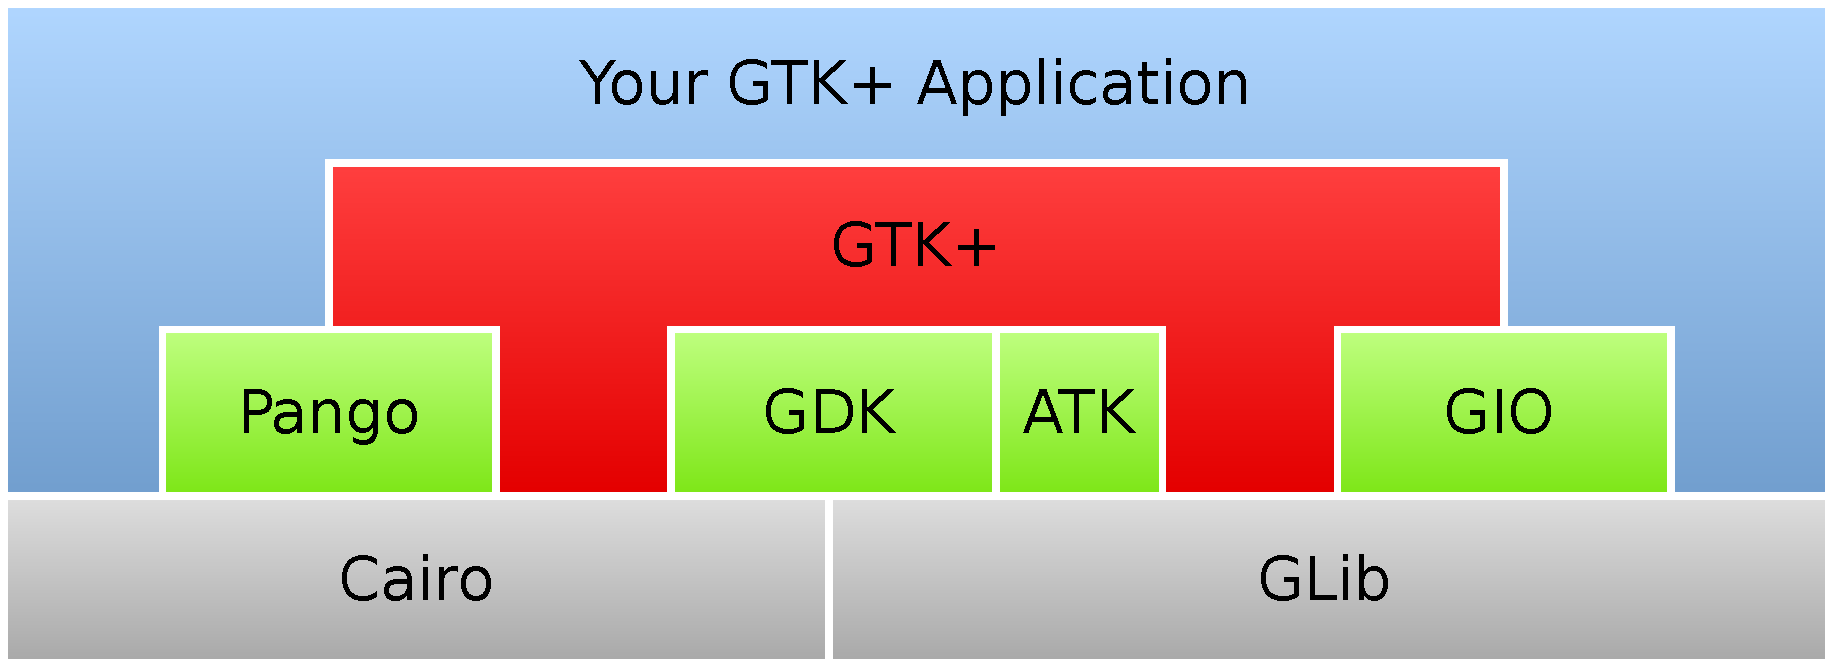
\includegraphics[width=\textwidth]{images/architecture.pdf}

\pagebreak
\section{GLib -- the Core Library}

Firstly, GLib provides common data structures:
\begin{itemize}
  \item Single and doubly linked lists.
  \item Hash tables.
  \item Balanced binary trees.
  \item N-ary trees: trees of data with any number of branches.
  \item Strings with text buffers which grow automatically as text is added.
  \item Arrays of arbitrary elements which grow automatically as elements are added.
  \item \texttt{GVariant}, a generic data type that stores a value along with information about the type of that value.
  \item And a few other data structures.
\end{itemize}

\bigskip
GLib also contains loads of utilities:
\begin{itemize}
  \item String and Unicode manipulation.
  \item Date and time functions.
  \item A command-line option parser.
  \item Perl-compatible regular expressions.
  \item An XML parser.
  \item A unit-test framework.
  \item And many other utilities.
\end{itemize}

\bigskip
Last, but not least, GLib provides some core event-driven programming features, with a \textit{main event loop}, support for threads and asynchronous communication between threads. An event loop listens some sources of events, that can come from file descriptors (plain files, pipes or sockets), timeouts, or other custom sources. A priority is associated with each source of events. When an event arrives, the event loop dispatches it to the application. The event can then be taken into account, either in the same thread or another thread.

\begin{center}
  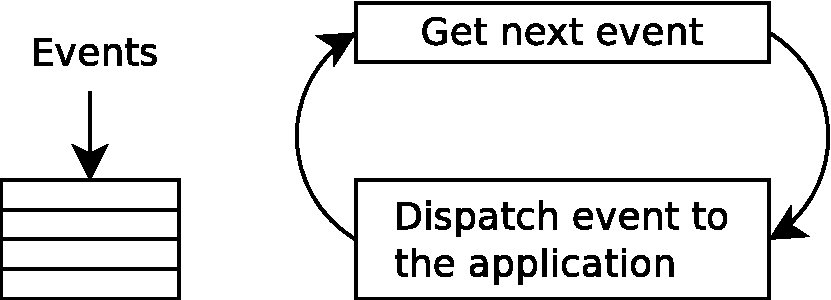
\includegraphics[width=6cm]{images/event-loop.pdf}\\[0.2cm]
  A main event loop.
\end{center}

\section{GObject -- an Object System}

Most modern programming languages come with their own native object systems and additional fundamental algorithmic language constructs. Just as GLib serves as an implementation of such fundamental types and algorithms (linked lists, hash tables and so forth), GObject provides an implementation of a flexible, extensible, and intentionally easy to map (into other languages) object-oriented framework for C.

All common object-oriented concepts are present: inheritance, interfaces, virtual/overridable methods, abstract classes, constructors, destructors, and so on. Memory management is handled by reference counting: when the reference count decreases to 0 the object is destroyed. GObject also provides a powerful \textit{signal system}: you can create your own signals and connect callback functions to it. It is a great way to decouple classes since the object sending the signal doesn't know who receive it. Another peculiarity of GObject is a \textit{property}, which is basically an object attribute surmounted by a \texttt{notify} signal that is sent when its value changes.

Alongside a GLib event loop, the GObject signal system forms a foundation for event-driven programming. The event-driven paradigm is not only useful for graphical user interfaces (with user events such as key presses and mouse clicks), but also for daemons that respond to hardware changes (a USB stick inserted, a second monitor connected, a printer low on paper), or software that listen to network connections or messages from other processes, among other examples.

\section{GIO -- Input/Output on Steroids}

GIO is striving to provide a modern, easy-to-use Virtual File System (VFS) API that sits at the right level in the library stack. GIO also contains other generally useful APIs for desktop applications (such as networking and D-Bus support). It was created to provide an API that is so good that developers prefer it over raw POSIX calls. Among other things that means using GObject. It also means not cloning the POSIX API, but providing higher-level, document-centric interfaces.

The abstract file system model of GIO consists of a number of interfaces and base classes for I/O and files. Then there is a number of stream classes, similar to the input and output stream hierarchies that can be found in frameworks like Java. There is a framework for storing and retrieving application settings. There is support for network programming, including connectivity monitoring, name resolution, lowlevel socket APIs and highlevel client and server helper classes. There is support for connecting to the D-Bus inter-process communication system: sending and receiving messages, owning and watching bus names, and making objects available on the bus. Beyond these, GIO provides: file monitoring; utility classes to implement asynchronous and/or cancellable operations; an easy-to-use API to launch and interact with child processes; and more.

In addition to the interfaces, GIO provides implementations for the local case. Implementations for various network file systems are provided by the GVFS package as loadable modules. Another design choice is to move backends out-of-process, which minimizes the dependency bloat and makes the whole system more robust. The backends are not included in GIO, but in the separate GVFS package. GVFS also contains a daemon which spawn further mount daemons for each individual connection.

\pagebreak
\section{The GTK+ Widget Toolkit}

On top of GLib/GObject/GIO sits GTK+, a library containing a wide range of \textit{widgets}. A widget is a basic component of a graphical user interface, for instance a button, some text, a menu, etc. A \textit{container} is a special widget that can contain other widgets. All these widgets are (indirect) subclasses of the \texttt{GObject} base class.

Although widgets can be created, configured and assembled programmatically, the Glade interface builder can be used to create the user interface graphically. The Glade application creates an XML file that can be loaded with GTK+.

Among other things, GTK+ provides a flexible theming system with a CSS-like language, as well as an interactive inspector.

\section{Long-Term Support GTK+ Versions}

During the GTK+~3 development, a new minor version was released every six months. GTK+~3.22 --~released in September 2016~-- is and will be the last minor version of the 3.x series. Moving forward, the GTK+ project has adopted a new versioning scheme with a new Long-Term Support (LTS) version released every two to three years. GTK+~3.22 is an LTS version, the next LTS version will be GTK+~4.0, then 5.0, etc. Intermediary versions will continue to be released every six months; for GTK+~4, those intermediary versions are numbered 3.90, 3.92, 3.94 and so on. Those non-LTS versions have less stability guarantees. Developers preferring a stable foundation should choose an LTS version of GTK+. An LTS version is supported at least three years.

% \section{Release Schedule and Versioning Scheme}
%
% The GTK+ project usually follows the GNOME release schedule, that is, new stable versions are released every six months, around March and September. A version number has the form X.Y.Z, where ``Y'' is even for stable versions and is odd for unstable versions. A new minor stable version (e.g. 3.14.0 $\rightarrow$ 3.14.1) doesn't add new features, only translation updates, bug fixes and performance improvements. For a library, a new major version number (``X'' in X.Y.Z) generally means there has been an API break. To address this, previous major versions are parallel-installable with the latest version.
%
% It's of course recommended to use the latest versions for newly-written code.

\section{More Information}

\url{https://www.gtk.org/}\\
\url{https://blog.gtk.org/}

\end{document}
